\documentclass[
  shownotes,
  xcolor={svgnames},
  hyperref={colorlinks,citecolor=DarkBlue,linkcolor=DarkRed,urlcolor=DarkBlue}
  , aspectratio=169]{beamer}
\usepackage{animate}
\usepackage{amsmath}
\usepackage{amsfonts}
\usepackage{amssymb}
\usepackage{pifont}
\usepackage{mathpazo}
%\usepackage{xcolor}
\usepackage{multimedia}
\usepackage{fancybox}
\usepackage[para]{threeparttable}
\usepackage{multirow}
\setcounter{MaxMatrixCols}{30}
\usepackage{subcaption}
\usepackage{graphicx}
\usepackage{lscape}
\usepackage[compatibility=false,font=small]{caption}
\usepackage{booktabs}
\usepackage{ragged2e}
\usepackage{chronosys}
\usepackage{appendixnumberbeamer}
\usepackage{animate}
\setbeamertemplate{caption}[numbered]
\usepackage{color}
%\usepackage{times}
\usepackage{tikz}
\usepackage{comment} %to comment
%% BibTeX settings
\usepackage{natbib}
\bibliographystyle{apalike}
\bibpunct{(}{)}{,}{a}{,}{,}
\setbeamertemplate{bibliography item}{[\theenumiv]}

% Defines columns for bespoke tables
\usepackage{array}
\newcolumntype{L}[1]{>{\raggedright\let\newline\\\arraybackslash\hspace{0pt}}m{#1}}
\newcolumntype{C}[1]{>{\centering\let\newline\\\arraybackslash\hspace{0pt}}m{#1}}
\newcolumntype{R}[1]{>{\raggedleft\let\newline\\\arraybackslash\hspace{0pt}}m{#1}}


\usepackage{xfrac}


\usepackage{multicol}
\setlength{\columnsep}{0.5cm}

% Theme and colors
\usetheme{Boadilla}

% I use steel blue and a custom color palette. This defines it.
\definecolor{andesred}{HTML}{af2433}

% Other options
\providecommand{\U}[1]{\protect\rule{.1in}{.1in}}
\usefonttheme{serif}
\setbeamertemplate{itemize items}[default]
\setbeamertemplate{enumerate items}[square]
\setbeamertemplate{section in toc}[circle]

\makeatletter

\definecolor{mybackground}{HTML}{82CAFA}
\definecolor{myforeground}{HTML}{0000A0}

\setbeamercolor{normal text}{fg=black,bg=white}
\setbeamercolor{alerted text}{fg=red}
\setbeamercolor{example text}{fg=black}

\setbeamercolor{background canvas}{fg=myforeground, bg=white}
\setbeamercolor{background}{fg=myforeground, bg=mybackground}

\setbeamercolor{palette primary}{fg=black, bg=gray!30!white}
\setbeamercolor{palette secondary}{fg=black, bg=gray!20!white}
\setbeamercolor{palette tertiary}{fg=white, bg=andesred}

\setbeamercolor{frametitle}{fg=andesred}
\setbeamercolor{title}{fg=andesred}
\setbeamercolor{block title}{fg=andesred}
\setbeamercolor{itemize item}{fg=andesred}
\setbeamercolor{itemize subitem}{fg=andesred}
\setbeamercolor{itemize subsubitem}{fg=andesred}
\setbeamercolor{enumerate item}{fg=andesred}
\setbeamercolor{item projected}{bg=gray!30!white,fg=andesred}
\setbeamercolor{enumerate subitem}{fg=andesred}
\setbeamercolor{section number projected}{bg=gray!30!white,fg=andesred}
\setbeamercolor{section in toc}{fg=andesred}
\setbeamercolor{caption name}{fg=andesred}
\setbeamercolor{button}{bg=gray!30!white,fg=andesred}


\usepackage{fancyvrb}
\newcommand{\VerbBar}{|}
\newcommand{\VERB}{\Verb[commandchars=\\\{\}]}
\DefineVerbatimEnvironment{Highlighting}{Verbatim}{commandchars=\\\{\}}
% Add ',fontsize=\small' for more characters per line
\usepackage{framed}
\definecolor{shadecolor}{RGB}{248,248,248}
\newenvironment{Shaded}{\begin{snugshade}}{\end{snugshade}}
\newcommand{\AlertTok}[1]{\textcolor[rgb]{0.94,0.16,0.16}{#1}}
\newcommand{\AnnotationTok}[1]{\textcolor[rgb]{0.56,0.35,0.01}{\textbf{\textit{#1}}}}
\newcommand{\AttributeTok}[1]{\textcolor[rgb]{0.77,0.63,0.00}{#1}}
\newcommand{\BaseNTok}[1]{\textcolor[rgb]{0.00,0.00,0.81}{#1}}
\newcommand{\BuiltInTok}[1]{#1}
\newcommand{\CharTok}[1]{\textcolor[rgb]{0.31,0.60,0.02}{#1}}
\newcommand{\CommentTok}[1]{\textcolor[rgb]{0.56,0.35,0.01}{\textit{#1}}}
\newcommand{\CommentVarTok}[1]{\textcolor[rgb]{0.56,0.35,0.01}{\textbf{\textit{#1}}}}
\newcommand{\ConstantTok}[1]{\textcolor[rgb]{0.00,0.00,0.00}{#1}}
\newcommand{\ControlFlowTok}[1]{\textcolor[rgb]{0.13,0.29,0.53}{\textbf{#1}}}
\newcommand{\DataTypeTok}[1]{\textcolor[rgb]{0.13,0.29,0.53}{#1}}
\newcommand{\DecValTok}[1]{\textcolor[rgb]{0.00,0.00,0.81}{#1}}
\newcommand{\DocumentationTok}[1]{\textcolor[rgb]{0.56,0.35,0.01}{\textbf{\textit{#1}}}}
\newcommand{\ErrorTok}[1]{\textcolor[rgb]{0.64,0.00,0.00}{\textbf{#1}}}
\newcommand{\ExtensionTok}[1]{#1}
\newcommand{\FloatTok}[1]{\textcolor[rgb]{0.00,0.00,0.81}{#1}}
\newcommand{\FunctionTok}[1]{\textcolor[rgb]{0.00,0.00,0.00}{#1}}
\newcommand{\ImportTok}[1]{#1}
\newcommand{\InformationTok}[1]{\textcolor[rgb]{0.56,0.35,0.01}{\textbf{\textit{#1}}}}
\newcommand{\KeywordTok}[1]{\textcolor[rgb]{0.13,0.29,0.53}{\textbf{#1}}}
\newcommand{\NormalTok}[1]{#1}
\newcommand{\OperatorTok}[1]{\textcolor[rgb]{0.81,0.36,0.00}{\textbf{#1}}}
\newcommand{\OtherTok}[1]{\textcolor[rgb]{0.56,0.35,0.01}{#1}}
\newcommand{\PreprocessorTok}[1]{\textcolor[rgb]{0.56,0.35,0.01}{\textit{#1}}}
\newcommand{\RegionMarkerTok}[1]{#1}
\newcommand{\SpecialCharTok}[1]{\textcolor[rgb]{0.00,0.00,0.00}{#1}}
\newcommand{\SpecialStringTok}[1]{\textcolor[rgb]{0.31,0.60,0.02}{#1}}
\newcommand{\StringTok}[1]{\textcolor[rgb]{0.31,0.60,0.02}{#1}}
\newcommand{\VariableTok}[1]{\textcolor[rgb]{0.00,0.00,0.00}{#1}}
\newcommand{\VerbatimStringTok}[1]{\textcolor[rgb]{0.31,0.60,0.02}{#1}}
\newcommand{\WarningTok}[1]{\textcolor[rgb]{0.56,0.35,0.01}{\textbf{\textit{#1}}}}
\usepackage{graphicx}
\makeatletter

\definecolor{airforceblue}{rgb}{0.36, 0.54, 0.66}

\usepackage{tikz}
% Tikz settings optimized for causal graphs.
\usetikzlibrary{shapes,decorations,arrows,calc,arrows.meta,fit,positioning}
\tikzset{
    -Latex,auto,node distance =1 cm and 1 cm,semithick,
    state/.style ={ellipse, draw, minimum width = 0.7 cm},
    point/.style = {circle, draw, inner sep=0.04cm,fill,node contents={}},
    bidirected/.style={Latex-Latex,dashed},
    el/.style = {inner sep=2pt, align=left, sloped}
}


\makeatother






%%%%%%%%%%%%%%% BEGINS DOCUMENT %%%%%%%%%%%%%%%%%%

\begin{document}

\title[Lecture 07]{Lecture 07: \\ Intro a Deep Learning, Redes Neuronales }
\subtitle{Aprendizaje y Minería de Datos para los Negocios}
\date{\today}

\author[Sarmiento-Barbieri]{Ignacio Sarmiento-Barbieri}
\institute[Uniandes]{Universidad de los Andes}


\begin{frame}[noframenumbering]
\maketitle
\end{frame}

%%%%%%%%%%%%%%%%%%%%%%%%%%%%%%%%%%%



%----------------------------------------------------------------------% 

\begin{frame}
\frametitle{Agenda}

\tableofcontents

\end{frame}
%----------------------------------------------------------------------%
\section{Recap}
%----------------------------------------------------------------------%
\begin{frame}
\frametitle{Deep Learning: Recap}
  
  \begin{itemize}
    \item Let's start with a familiar and simple model, the linear model
  
  \end{itemize}

\def\layersep{2.5cm}

\begin{align}
y &= f(X) + u \\ \nonumber
y &= \beta_1 x_1 + \beta_2 x_2 + \beta_3 x_3  + u
\end{align}


\begin{figure}[H]
\centering

\begin{tikzpicture}[shorten >=1pt,->,draw=black!50, node distance=\layersep]
    \tikzstyle{every pin edge}=[<-,shorten <=1pt]
    \tikzstyle{neuron}=[circle,fill=black!25,minimum size=17pt,inner sep=0pt]
    \tikzstyle{input neuron}=[neuron, fill=green!50];
    \tikzstyle{output neuron}=[neuron, fill=red!50];
    \tikzstyle{annot} = [text width=4em, text centered]

    % Draw the input layer nodes
    \foreach \name / \y in {1,...,3}
    % This is the same as writing \foreach \name / \y in {1/1,2/2,3/3,4/4}
        \node[input neuron, pin=left:$x_\y$] (I-\name) at (0,-\y) {};

    % Draw the output layer node
    \node[output neuron,pin={[pin edge={->}]right:y}, right of=I-2] (O) {};

    % Connect every node in the input layer with every node in the
    % hidden layer.
    

    % Connect every node in the hidden layer with the output layer
    \foreach \source in {1,...,3}
        \path (I-\source) edge (O);

    \node[annot,above of=I-1, node distance=1cm] (i) {Input layer};
    \node[annot,right of=i] {Output layer};

\end{tikzpicture}
\end{figure}



\end{frame}
%----------------------------------------------------------------------%
\section{Multilayer Perceptrons}
%----------------------------------------------------------------------%
\begin{frame}
\frametitle{Multilayer Perceptrons}

\begin{itemize}
    \item Linear Models may be to simple, and miss the nonlinearities that best approximate $f^*(x)$
    \medskip
    \item We can overcome these limitations of linear models and handle a more general class of functions by incorporating one or more hidden layers.
    \medskip
    \item Deep feedforward networks, also called feedforward neural networks, or
multilayer perceptrons (MLPs), are the quintessential deep learning models
\medskip
\item Feedforward neural networks are called
networks because they are typically represented by composing together many different functions. 
\item The model is associated with a directed acyclic graph describing how the functions are composed together. For example, we might have two functions $f^{(2)}$, $f^{(1)}$ and connected in a chain to form $f(x)=f^{(2)}(f^{(1)}(x))$ and
 \item These chain structures are the most commonly used structures of neural networks. 
\end{itemize}
\end{frame}

%----------------------------------------------------------------------%
\begin{frame}
\frametitle{Multilayer Perceptrons}


\def\layersep{2.5cm}

\begin{figure}[H]
\centering
\begin{tikzpicture}[shorten >=1pt,->,draw=black!50, node distance=\layersep]
    \tikzstyle{every pin edge}=[<-,shorten <=1pt]
    \tikzstyle{neuron}=[circle,fill=black!25,minimum size=17pt,inner sep=0pt]
    \tikzstyle{input neuron}=[neuron, fill=green!50];
    \tikzstyle{output neuron}=[neuron, fill=red!50];
    \tikzstyle{hidden neuron}=[neuron, fill=blue!50];
    \tikzstyle{annot} = [text width=4em, text centered]

    % Draw the input layer nodes
    \foreach \name / \y in {1,...,4}
    % This is the same as writing \foreach \name / \y in {1/1,2/2,3/3,4/4}
        \node[input neuron, pin=left: $x_\y$] (I-\name) at (0,-\y) {};

    % Draw the hidden layer nodes
    \foreach \name / \y in {1,...,5}
        \path[yshift=0.5cm]
            node[hidden neuron] (H-\name) at (\layersep,-\y cm) {};

    % Draw the output layer node
    \node[output neuron,pin={[pin edge={->}]right:y}, right of=H-3] (O) {};

    % Connect every node in the input layer with every node in the
    % hidden layer.
    \foreach \source in {1,...,4}
        \foreach \dest in {1,...,5}
            \path (I-\source) edge (H-\dest);

    % Connect every node in the hidden layer with the output layer
    \foreach \source in {1,...,5}
        \path (H-\source) edge (O);

    % Annotate the layers
    \node[annot,above of=H-1, node distance=1cm] (hl) {Hidden layer};
    \node[annot,left of=hl] {Input layer};
    \node[annot,right of=hl] {Output layer};
\end{tikzpicture}
\end{figure}

\end{frame}
%----------------------------------------------------------------------%
\begin{frame}
\frametitle{Multilayer Perceptrons}


\begin{itemize}



\item The overall length of the chain gives the depth of the model. The name “deep learning” arose from this terminology. 
\medskip
\item The final layer of a feedforward network is called the
output layer
\medskip
\item During neural network training, we try to train $f(x)$ to match $f^*(x)$
\medskip
\item In the training data we observe the first layer, inputs ($x$), and the last layer, output ($y$)
\medskip
\item We do not observe the intermediate layers,they are then called hidden layers.
\medskip
\item Finally, these networks are called neural because they are loosely inspired by
neuroscience.



\end{itemize}
\end{frame}

%----------------------------------------------------------------------%
\subsection{Worked Example}
%----------------------------------------------------------------------%
\begin{frame}
\frametitle{Worked Example: The "Exclusive OR (XOR)" Function}
\begin{itemize}
\item The exclusive disjunction of a pair of propositions, (p, q), is supposed to mean that p is true or q is true, but not both
\item It's truth table is:

\begin{table}[H]
\begin{tabular}{lllll}
q  & p & q v p \\
\hline
0 & 0 & 0 \\
0 & 1 & 1 \\
1 & 0 & 1 \\
1 & 1 & 0 \\
\end{tabular}
\end{table}
\item When exactly one of these binary values is equal to 1, the XOR function
returns 1. Otherwise, it returns 0
\end{itemize}

\end{frame}
%----------------------------------------------------------------------%
\begin{frame}
\frametitle{Worked Example: The "Exclusive OR (XOR)" Function}

\begin{itemize}
\item Let's use a linear model 

\begin{align}
y = X\beta + \iota \alpha 
\end{align}


 \begin{align}
 y=\left(\begin{array}{c}
0\\
1\\
1\\
0
\end{array}\right)X=\left(\begin{array}{cc}
0 & 0\\
0 &1\\
1 & 0\\
1 & 1
\end{array}\right)\iota=\left(\begin{array}{c}
1\\
1\\
1\\
1
\end{array}\right)
 \end{align}

\item Solution $ \alpha=\frac{1}{2} \,\,\,\beta=\left(\begin{array}{c}
0\\
0
\end{array}\right)
$


\item Prediction $\hat{y}=\left(\begin{array}{c}
\frac{1}{2}\\
\frac{1}{2}\\
\frac{1}{2}\\
\frac{1}{2}
\end{array}\right)$
\end{itemize}


\end{frame}
%----------------------------------------------------------------------%
\begin{frame}
\frametitle{Worked Example: The "Exclusive OR (XOR)" Function}

\begin{itemize}
 \item Let's  use multilayer perceptrons (feedforward network) with one hidden
layer containing two hidden units


\def\layersep{2cm}

\begin{figure}[H]
\centering
\begin{tikzpicture}[shorten >=1pt,->,draw=black!50, node distance=\layersep]
    \tikzstyle{every pin edge}=[<-,shorten <=1pt]
    \tikzstyle{neuron}=[circle,fill=black!25,minimum size=17pt,inner sep=0pt]
    \tikzstyle{input neuron}=[neuron, fill=green!50];
    \tikzstyle{output neuron}=[neuron, fill=red!50];
    \tikzstyle{hidden neuron}=[neuron, fill=blue!50];
    \tikzstyle{annot} = [text width=4em, text centered]

    % Draw the input layer nodes
    \foreach \name / \y in {1,...,2}
    % This is the same as writing \foreach \name / \y in {1/1,2/2,3/3,4/4}
        \node[input neuron, pin=left: $x_\y$] (I-\name) at (0,-\y) {};

    % Draw the hidden layer nodes
    \foreach \name / \y in {1,...,2}
        \path[yshift=0cm]
            node[hidden neuron] (H-\name) at (\layersep,-\y cm) {};

    % Draw the output layer node
    \node[output neuron,yshift=-0.5cm, pin={[pin edge={->}]right:y}, right of=H-1] (O) {};

    % Connect every node in the input layer with every node in the
    % hidden layer.
    \foreach \source in {1,...,2}
        \foreach \dest in {1,...,2}
            \path (I-\source) edge (H-\dest);

    % Connect every node in the hidden layer with the output layer
    \foreach \source in {1,...,2}
        \path (H-\source) edge (O);

    % Annotate the layers
    \node[annot,above of=H-1, node distance=1cm] (hl) {Hidden layer};
    \node[annot,left of=hl] {Input layer};
    \node[annot,right of=hl] {Output layer};
\end{tikzpicture}
\end{figure}

\item This network has a vector of hidden units $h$ that are computed by a
function $f^{(1)}(x;W , c)$. 
\item The values of these hidden units are then used as the input for a second layer. \item The second layer is the output layer of the network. The output
layer is still just a linear regression model, but now it is applied to $h$ rather than to $x$
\item  The network now contains two functions chained together, $f(x;W , c, w, b) = f^{(2)}(f^{(1)}(x))$
\end{itemize}

\end{frame}
%----------------------------------------------------------------------%
\begin{frame}
\frametitle{Worked Example: The "Exclusive OR (XOR)" Function}

\begin{itemize}
    \item Which $f^{(1)}$ should we specify?
    \medskip
    \begin{itemize}
    \item Clearly {\bf not} linear, otherwise it would defeat the entire purpose
    \item We are going to use the rectified linear unit or ReLU (it is usually the default recommendation, there are many others (more on this later))
    \item ReLU is defined as $g(z)=max\{0,z\}$
    \end{itemize}
    
    \item For $f^{(2)}$? For this example, a linear model will suffice 
    \medskip
    \begin{align}
    f^{(2)} = f^{(1)}w + b
    \end{align}
    \item The final model is then 
    \begin{align}
    f(x,W,C,w,b) = max\{0,XW+c\}\,w + b
    \end{align}
\end{itemize}

\end{frame}
%----------------------------------------------------------------------%
\begin{frame}
\frametitle{Worked Example: The "Exclusive OR (XOR)" Function}

\begin{itemize}
\item Suppose this is the solution to the XOR problem 
\end{itemize}


\[
f(x)=max\{0,XW+c\}\,w+b
\]

\[
W=\left(\begin{array}{cc}
1 & 1\\
1 & 1
\end{array}\right)
\]

\[
c=\left(\begin{array}{cc}
0 & -1\\
0 & -1\\
0 & -1\\
0 & -1
\end{array}\right)
\]

\[
w=\left(\begin{array}{cc}
1 & -2\end{array}\right)
\]

 \[
 b = 0
 \]


\end{frame}
%----------------------------------------------------------------------%
\begin{frame}
\frametitle{Worked Example: The "Exclusive OR (XOR)" Function}

\begin{itemize}
\item Lets work out the example step by step
\end{itemize}
\begin{align}
f(x)=max\{0,XW+c\}\,w+b
\end{align}

\[
XW=\left(\begin{array}{cc}
0 & 0\\
0 & 0\\
1 & 0\\
1 & 0
\end{array}\right)\left(\begin{array}{cc}
1 & 1\\
1 & 1
\end{array}\right)=\left(\begin{array}{cc}
0 & 0\\
1 & 1\\
1 & 1\\
2 & 2
\end{array}\right)
\]

\[
XW+c=\left(\begin{array}{cc}
0 & -1\\
1 & 0\\
1 & 0\\
2 & 1
\end{array}\right)
\]

\[
max\{0,XW+c\}=\left(\begin{array}{cc}
0 & 0\\
1 & 0\\
1 & 0\\
2 & 1
\end{array}\right)
\]

\end{frame}
%----------------------------------------------------------------------%
\begin{frame}
\frametitle{Worked Example: The "Exclusive OR (XOR)" Function}


\[
\hat{y}=max\{0,XW+c\}\,w + b=\left(\begin{array}{cc}
0 & 0\\
1 & 0\\
1 & 0\\
2 & 1
\end{array}\right)\left(\begin{array}{cc}
1 & -2\end{array}\right)=\left(\begin{array}{c}
0\\
1\\
1\\
0
\end{array}\right)
\]

\vspace{2cm}
\begin{itemize}
\item The neural network has obtained the correct answer for every data point
\end{itemize}

\end{frame}
%----------------------------------------------------------------------%
\begin{frame}
\frametitle{Worked Example: The "Exclusive OR (XOR)" Function}

\begin{itemize}
\item In this example, we simply specified the solution, then showed that
it obtained zero error.
\item In a real situation, there might be billions of model parameters and
billions of training examples, so one cannot simply guess the solution
as we did here.
\item Instead, a gradient-based optimization algorithm can find parameters
that produce very little error. 
\item The solution we described to the XOR problem is at a global minimum
of the loss function, so gradient descent could converge to this point.
\item There are other equivalent solutions to the XOR problem that gradient
descent could also find. 
\item The convergence point of gradient descent depends on the initial values
of the parameters. 
\item In practice, gradient descent would usually not find clean, easily
understood, integer-valued solutions like the one we presented here.
\end{itemize}


\end{frame}


%----------------------------------------------------------------------%
\subsection{Minimalist Theory}
%----------------------------------------------------------------------%
\begin{frame}
\frametitle{Multilayer Perceptrons: Theory}

\begin{itemize}
 \item Why not a linear model? 


\begin{align} 
 \mathbf{H} & = \mathbf{X} \mathbf{W}^{(1)} + \mathbf{b}^{(1)} \\ \nonumber
 \mathbf{Y} & = \mathbf{H}\mathbf{W}^{(2)} + \mathbf{b}^{(2)}  \nonumber
  \end{align} 
\bigskip
\item  where $\mathbf{X} \in \mathbb{R}^{n \times d}$,  $n$ obs. and $d$ inputs (features). 
\item H is a hidden layer with $h$ hidden units, $\mathbf{H} \in \mathbb{R}^{n \times h}$

\item  Because the hidden and output layers are both fully connected, we have 
\begin{itemize}
 \item hidden-layer weights $\mathbf{W}^{(1)} \in \mathbb{R}^{d \times h}$ and biases $\mathbf{b}^{(1)} \in \mathbb{R}^{1 \times h}$  
\item output-layer weights $\mathbf{W}^{(2)} \in \mathbb{R}^{h \times q}$ and biases $\mathbf{b}^{(2)} \in \mathbb{R}^{1 \times q}$
\end{itemize}

\end{itemize}

\end{frame}
%----------------------------------------------------------------------%
\begin{frame}
\frametitle{Multilayer Perceptrons: Theory}

\begin{itemize}
 \item Why not a linear model?
\medskip
\item Note that after adding the linear hidden layer , we gain nothing for our troubles! 
\medskip


\begin{align}
\mathbf{Y} &= (\mathbf{X} \mathbf{W}^{(1)} + \mathbf{b}^{(1)})\mathbf{W}^{(2)} + \mathbf{b}^{(2)} \\ \nonumber
&= \mathbf{X} \mathbf{W}^{(1)}\mathbf{W}^{(2)} + \mathbf{b}^{(1)} \mathbf{W}^{(2)} + \mathbf{b}^{(2)} \\ \nonumber
&= \mathbf{X} \mathbf{W} + \mathbf{b}. \nonumber
\end{align} 
\end{itemize}

\end{frame}
%----------------------------------------------------------------------%
\begin{frame}
\frametitle{Multilayer Perceptrons: Theory}

\begin{itemize}
    \item The gain comes from using nonlinear activation function $\sigma$
    \item Note that, with activation functions in place, it is no longer possible to collapse our MLP into a linear model:

 \begin{align} 
 \mathbf{H} & = \sigma(\mathbf{X} \mathbf{W}^{(1)} + \mathbf{b}^{(1)}), \\ \nonumber
 \mathbf{Y} & = \mathbf{H}\mathbf{W}^{(2)} + \mathbf{b}^{(2)}.
 \end{align} 

\item Note that we can build more general MLPs, by stacking hidden layers, yielding ever more expressive models.

\begin{align}
\mathbf{H}^{(1)} &= \sigma_1(\mathbf{X} \mathbf{W}^{(1)} + \mathbf{b}^{(1)}) \\ \nonumber
\mathbf{H}^{(2)} &= \sigma_2(\mathbf{H}^{(1)} \mathbf{W}^{(2)} + \mathbf{b}^{(2)}) \\ \nonumber
\mathbf{Y} & = \mathbf{H}^{2}\mathbf{W}^{(3)} + \mathbf{b}^{(3)}.
\end{align}


\end{itemize}

\end{frame}
%----------------------------------------------------------------------%
\subsubsection{Activation Functions}
%----------------------------------------------------------------------%
\begin{frame}
\frametitle{Activation Functions}

\begin{itemize}
\item Activation functions are fundamental to deep learning, let us briefly survey some common activation functions.
\medskip
\item ReLU Function
\begin{itemize}
\item The most popular choice, due to both simplicity of implementation and its good performance on a variety of predictive tasks, is the rectified linear unit (ReLU). 
\medskip
\item ReLU provides a very simple nonlinear transformation. Given an element $x$, the function is defined as the maximum of that element and $0$:

$$\operatorname{ReLU}(x) = \max \{x, 0\}.$$

\end{itemize}
\end{itemize}

\end{frame}
%----------------------------------------------------------------------%
\begin{frame}
\frametitle{Activation Functions}

\begin{itemize}
\item  ReLU function retains only positive elements and discards all negative elements by setting the corresponding activations to 0. 
\item It is piecewise linear.
\end{itemize}



  \begin{figure}[H] \centering
            \captionsetup{justification=centering}
              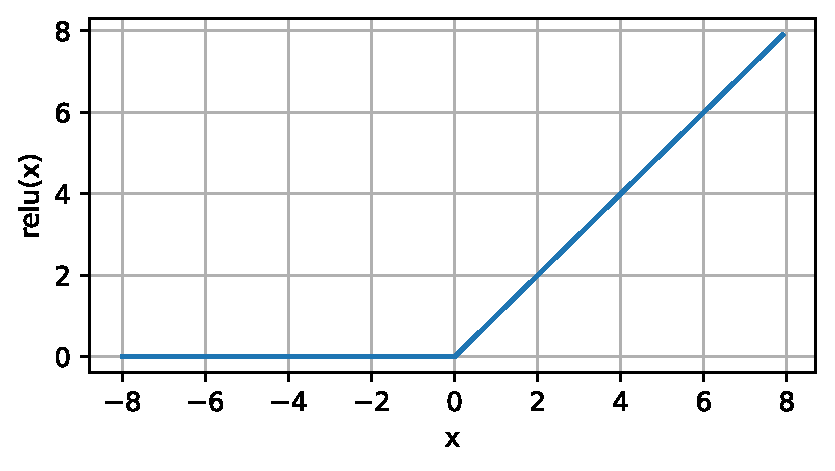
\includegraphics[scale=0.45]{figures/relu}
              
 \end{figure}

\end{frame}
%----------------------------------------------------------------------%
\begin{frame}
\frametitle{Activation Functions}
\begin{itemize}
    \item Part of the appeal of ReLU has to do with it's well behaved derivative
    \begin{itemize}
        \item  Note that the ReLU function is not differentiable when the input takes value precisely equal to 0. In these cases, we default to the left-hand-side derivative and say that the derivative is 0 when the input is 0. ( we may even get away with this because the input may never actually be zero!)
        \item This makes optimization better behaved and it mitigates the problem of vanishing gradients
    \end{itemize}
    
\end{itemize}



  \begin{figure}[H] \centering
            \captionsetup{justification=centering}
              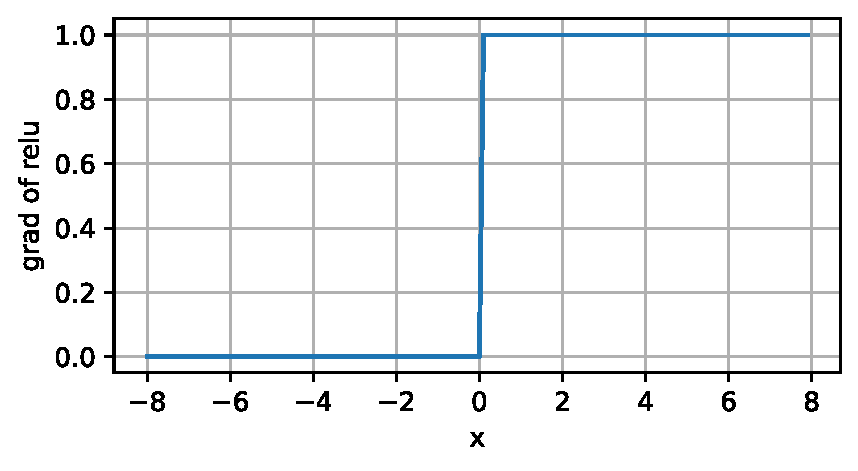
\includegraphics[scale=0.45]{figures/relu_dev}
              
 \end{figure}


\end{frame}
%----------------------------------------------------------------------%
\begin{frame}
\frametitle{Activation Functions}





\begin{itemize}

\item Sigmoid Function

\begin{itemize}



\item The sigmoid function transforms its inputs, for which values lie in the domain $\mathbb{R}$, to outputs that lie on the interval (0, 1). 
\item For that reason, the sigmoid is often called a squashing function: it squashes any input in the range (-inf, inf) to some value in the range (0, 1):

$$\operatorname{sigmoid}(x) = \frac{1}{1 + \exp(-x)}.$$

\item In the earliest neural networks, scientists were interested in modeling biological neurons which either fire or do not fire. Thus the pioneers of this field, going all the way back to McCulloch and Pitts, the inventors of the artificial neuron, focused on thresholding units. A thresholding activation takes value 0 when its input is below some threshold and value 1 when the input exceeds the threshold.

\item When attention shifted to gradient based learning, the sigmoid function was a natural choice because it is a smooth, differentiable approximation to a thresholding unit. 

    \end{itemize}
\end{itemize}    



\end{frame}
%----------------------------------------------------------------------%
\begin{frame}
\frametitle{Activation Functions}




\begin{itemize}

\item Sigmoid Function

\end{itemize}

  \begin{figure}[H] \centering
            \captionsetup{justification=centering}
              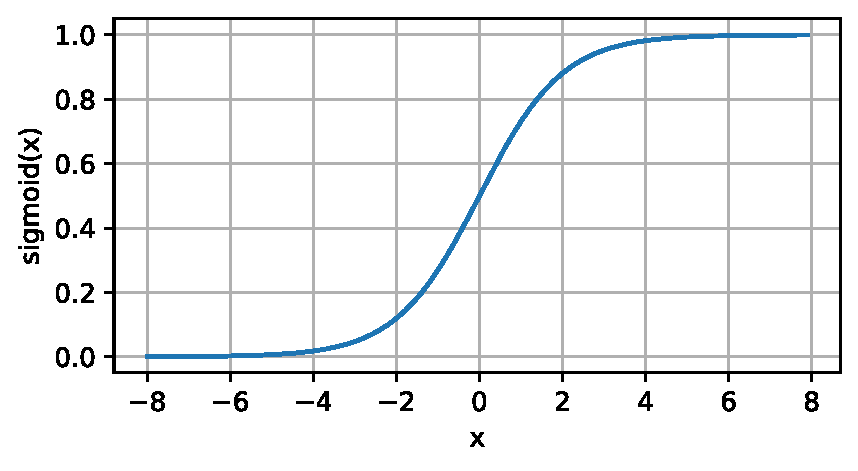
\includegraphics[scale=0.45]{figures/sigmoid}
              
 \end{figure}

\end{frame}

%----------------------------------------------------------------------%
\begin{frame}
\frametitle{Activation Functions}

\begin{itemize}
\item The derivative of the sigmoid function is given by the following equation:

$$\frac{d}{dx} \operatorname{sigmoid}(x) = \frac{\exp(-x)}{(1 + \exp(-x))^2} = \operatorname{sigmoid}(x)\left(1-\operatorname{sigmoid}(x)\right).$$

\end{itemize}




  \begin{figure}[H] \centering
            \captionsetup{justification=centering}
              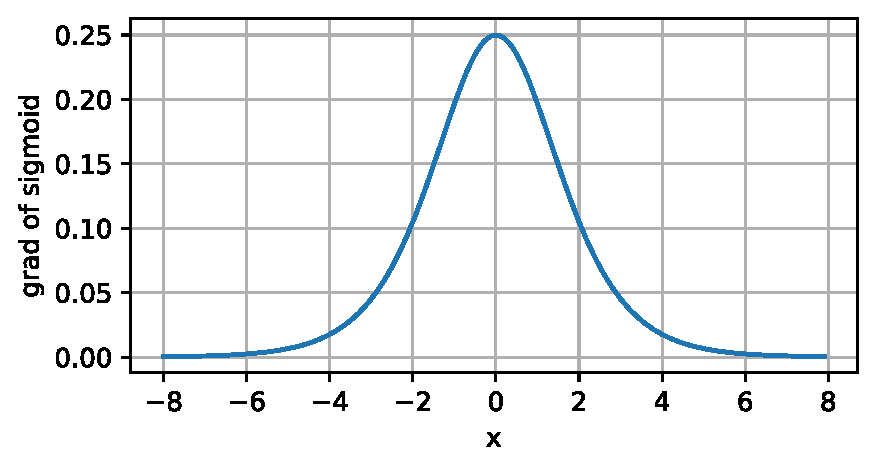
\includegraphics[scale=0.45]{figures/sigmoid_dev}
              
 \end{figure}

\end{frame}

%----------------------------------------------------------------------%
\begin{frame}
\frametitle{Activation Functions}




\begin{itemize}
    
\item $Tanh$ Function
  \begin{itemize}
        \item Like the sigmoid function, the tanh (hyperbolic tangent) function also squashes its inputs, transforming them into elements on the interval between -1 and 1:

        $$\operatorname{tanh}(x) = \frac{1 - \exp(-2x)}{1 + \exp(-2x)}.$$

        \item Although the shape of the function is similar to that of the sigmoid function, the $tanh$ function exhibits point symmetry about the origin of the coordinate system.
    \end{itemize}
\end{itemize}

  \begin{figure}[H] \centering
            \captionsetup{justification=centering}
              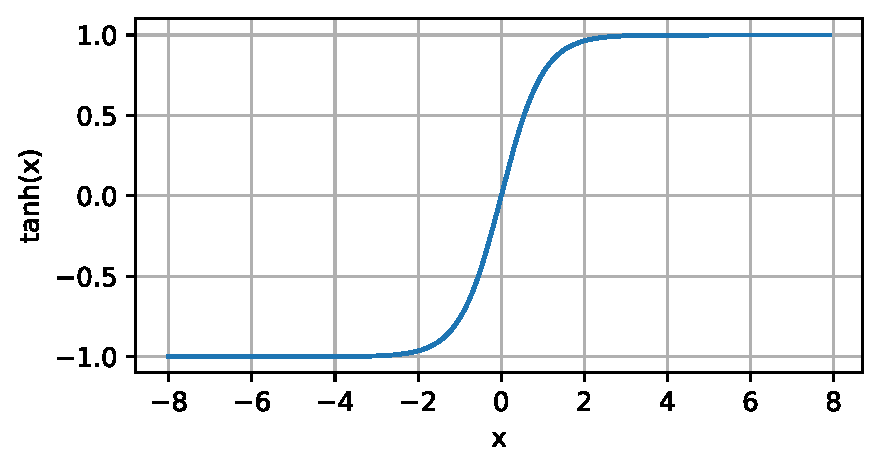
\includegraphics[scale=0.45]{figures/tanh}
              
 \end{figure}

\end{frame}

%----------------------------------------------------------------------%
\begin{frame}
\frametitle{Activation Functions}

\begin{itemize}
\item The derivative of the $tanh$ function is:

$$\frac{d}{dx} \operatorname{tanh}(x) = 1 - \operatorname{tanh}^2(x).$$

\item The derivative of $tanh$ function is plotted below. As the input nears 0, the derivative of the $tanh$ function approaches a maximum of 1. And as we saw with the sigmoid function, as the input moves away from 0 in either direction, the derivative of the $tanh$ function approaches 0.
\end{itemize}


  \begin{figure}[H] \centering
            \captionsetup{justification=centering}
              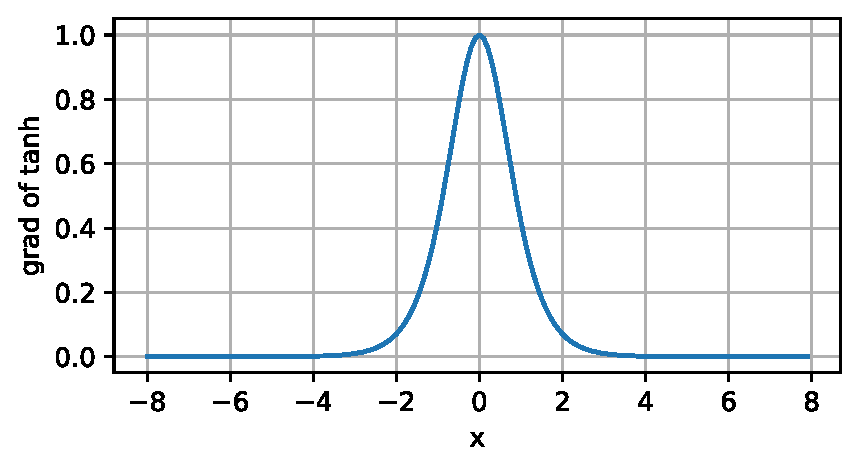
\includegraphics[scale=0.45]{figures/tanh_dev}
              
 \end{figure}



\end{frame}
%----------------------------------------------------------------------%
\begin{frame}
\frametitle{Activation Functions}


\begin{itemize}
\item Other Activation functions
\medskip
\begin{itemize}
\item $h=cos(W x+b)$ Goodfellow et all (2016) claim that on the MNIST dataset they obtained an error rate of less than 1 percent
\medskip
\item Radial basis function (RBF): $exp\left( \frac{1}{\sigma^2)}||W-x||^2 \right)$
\medskip
\item Softplus: $log(1+e^x)$
\medskip
\item Hard tanh: $max(-1,min(1,x))$
\medskip
\end{itemize}
\item Hidden unit design remains an active area of research, and many useful hidden unit types remain to be discovered
\end{itemize}


\end{frame}
%----------------------------------------------------------------------%
\subsubsection{Output Functions}
%----------------------------------------------------------------------%
\begin{frame}
\frametitle{Output Functions}

\begin{itemize}
\item The choice of cost function is tightly coupled with the choice of output unit. 
\medskip
\item Most of the time, we simply use the distance between the data distribution and the model distribution. 
\medskip
\begin{itemize}

    \item Linear $y=W'h +b$ $\rightarrow$  $\mathbb{R}$
    \medskip
    \item Sigmoid (Logistic)$\frac{1}{1 + \exp(-x)}$ $\rightarrow$ classification $\{0,1\}$
    \medskip
    \item Softmax $\frac{exp(x)}{\sum exp(x))}$ $\rightarrow$ classification multiple categories
\end{itemize}
\end{itemize}

\end{frame}


%----------------------------------------------------------------------%
\subsubsection{Architecture Design}
%----------------------------------------------------------------------%
\begin{frame}
\frametitle{Architecture Design}

\begin{itemize}


\item Another key design consideration for neural networks is determining the architecture.

\item The word architecture refers to the overall structure of the network: how many units it should have and how these units should be connected to each other.

\item In these chain-based architectures, the main architectural considerations are choosing the depth of the network and the width of each layer. 

\item A multilayer perceptron (feedforward networks) with hidden layers provide a universal approximation framework. 
\begin{itemize}
\item The universal approximation theorem (Hornik et al., 1989; Cybenko, 1989) states that a feedforward network with a linear output layer and at least one hidden layer with any “squashing” activation function (such as the logistic sigmoid activation function) can approximate any Borel measurable function from one finite-dimensional space to another with any desired nonzero amount of error, provided that the network is given enough hidden unit.

\item The derivatives of the feedforward network can also approximate the derivatives of the
function arbitrarily well (Hornik et al., 1990). 
\end{itemize}



\end{itemize}

\end{frame}
%----------------------------------------------------------------------%
\begin{frame}
\frametitle{Architecture Design}

\begin{itemize}

    \item The universal approximation theorem means that regardless of what function we are trying to learn, we know that a large MLP will be able to represent this function. 
    \item We are not guaranteed, however, that the training algorithm will be able to learn that function. Even if the MLP is able to represent the function, learning can fail for two different reasons. 
            \begin{enumerate}
                \item The optimization algorithm used
                for training may not be able to find the value of the parameters that corresponds
                to the desired function. 
                \item The training algorithm might choose the wrong function as a result of overfitting
            \end{enumerate}


    \item A feedforward network with a single layer is sufficient to represent any function, but the layer may be infeasible large and may fail to learn and generalize correctly.

    \item  In many circumstances, using deeper models can reduce the number of units required to represent the desired function and can reduce the amount of generalization error.
    \item  The ideal network architecture for a task must be found via experimentation guided by monitoring the validation set error
\end{itemize}
\end{frame}
%----------------------------------------------------------------------%
\subsubsection{Numerical Optimization Issues}
%----------------------------------------------------------------------%
\begin{frame}
\frametitle{Numerical Stability and Initialization}

\begin{itemize}
\item Vanishing and exploding gradients are common issues in deep networks. Great care in parameter initialization is required to ensure that gradients and parameters remain well controlled.
\medskip
\item Initialization heuristics are needed to ensure that the initial gradients are neither too large nor too small.
\medskip
\item ReLU activation functions mitigate the vanishing gradient problem. This can accelerate convergence.
\medskip
\item Random initialization is key to ensure that symmetry is broken before optimization
\end{itemize}

\end{frame}
%----------------------------------------------------------------------%
\subsection{Demo}
%----------------------------------------------------------------------%
\begin{frame}[fragile]
\frametitle{Deep Learning: Demo}





\begin{Shaded}
\begin{Highlighting}[]
\KeywordTok{library}\NormalTok{(keras)}
\NormalTok{fashion\_mnist \textless{}{-}}\StringTok{ }\KeywordTok{dataset\_fashion\_mnist}\NormalTok{()}
\end{Highlighting}
\end{Shaded}

  \begin{figure}[H] \centering
            \captionsetup{justification=centering}
              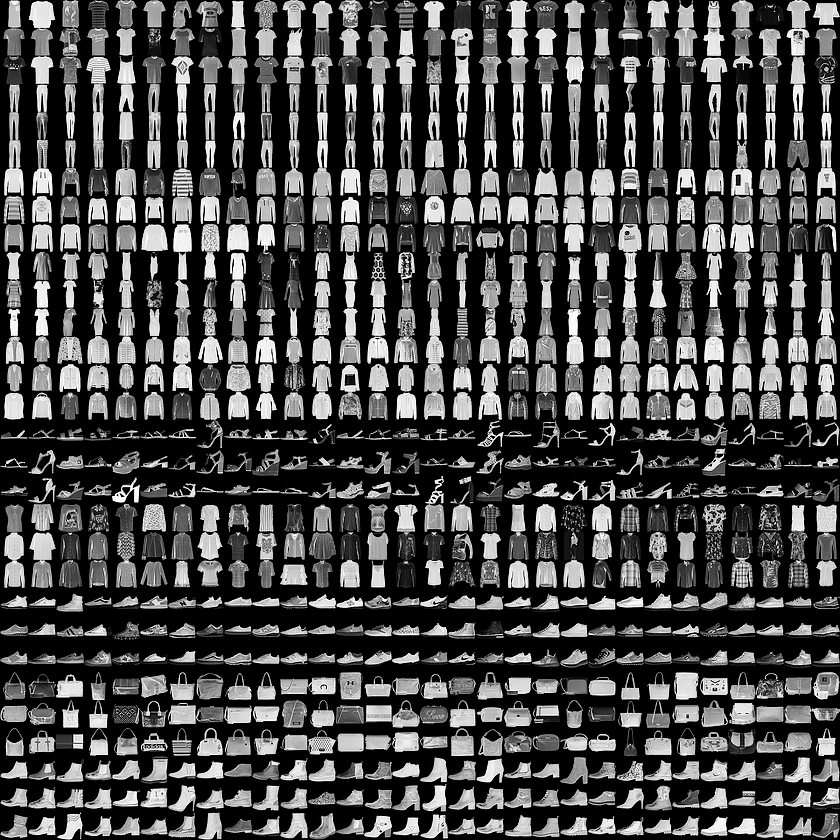
\includegraphics[scale=0.4]{figures/fashion-mnist-sprite}
              
 \end{figure}
\end{frame}
%----------------------------------------------------------------------%
\begin{frame}[fragile]
\frametitle{Deep Learning: Demo}

\begin{Shaded}
\begin{Highlighting}[]


\KeywordTok{c}\NormalTok{(train\_images, train\_labels) }\OperatorTok{\%\textless{}{-}\%}\StringTok{ }\NormalTok{fashion\_mnist}\OperatorTok{$}\NormalTok{train}
\KeywordTok{c}\NormalTok{(test\_images, test\_labels) }\OperatorTok{\%\textless{}{-}\%}\StringTok{ }\NormalTok{fashion\_mnist}\OperatorTok{$}\NormalTok{test}

\NormalTok{class\_names =}\StringTok{ }\KeywordTok{c}\NormalTok{(}\StringTok{\textquotesingle{}T{-}shirt/top\textquotesingle{}}\NormalTok{,}
                \StringTok{\textquotesingle{}Trouser\textquotesingle{}}\NormalTok{,}
                \StringTok{\textquotesingle{}Pullover\textquotesingle{}}\NormalTok{,}
                \StringTok{\textquotesingle{}Dress\textquotesingle{}}\NormalTok{,}
                \StringTok{\textquotesingle{}Coat\textquotesingle{}}\NormalTok{, }
                \StringTok{\textquotesingle{}Sandal\textquotesingle{}}\NormalTok{,}
                \StringTok{\textquotesingle{}Shirt\textquotesingle{}}\NormalTok{,}
                \StringTok{\textquotesingle{}Sneaker\textquotesingle{}}\NormalTok{,}
                \StringTok{\textquotesingle{}Bag\textquotesingle{}}\NormalTok{,}
                \StringTok{\textquotesingle{}Ankle boot\textquotesingle{}}\NormalTok{)}
\end{Highlighting}
\end{Shaded}

\end{frame}
%----------------------------------------------------------------------%
\begin{frame}[fragile]
\frametitle{Deep Learning: Demo}

\begin{Shaded}
\begin{Highlighting}[]
\NormalTok{train\_images \textless{}{-}}\StringTok{ }\NormalTok{train\_images }\OperatorTok{/}\StringTok{ }\DecValTok{255}
\NormalTok{test\_images \textless{}{-}}\StringTok{ }\NormalTok{test\_images }\OperatorTok{/}\StringTok{ }\DecValTok{255}
\end{Highlighting}
\end{Shaded}

  \begin{figure}[H] \centering
            \captionsetup{justification=centering}
              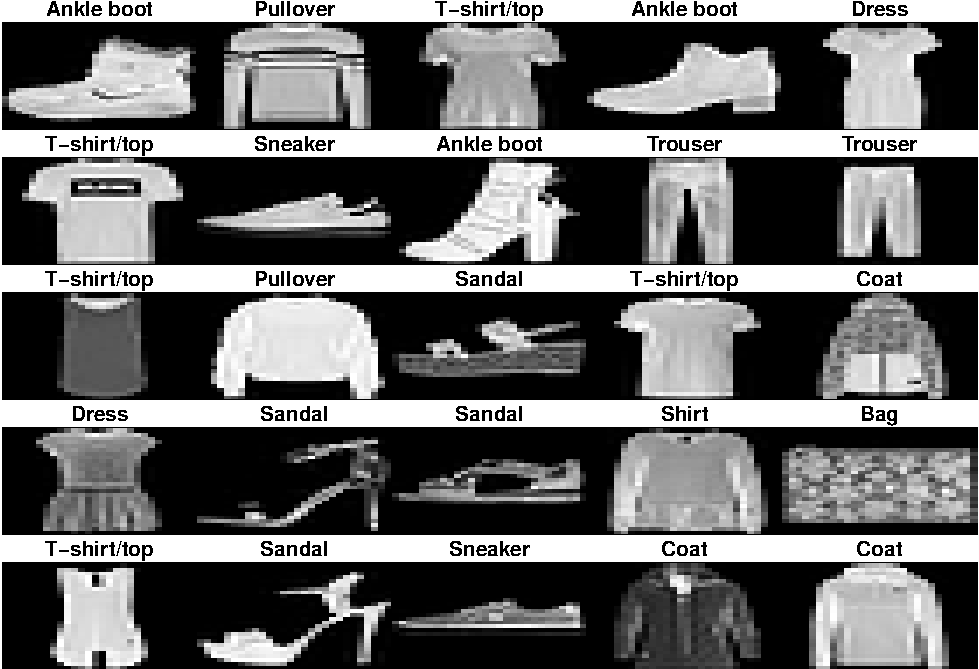
\includegraphics[scale=0.4]{figures/unnamed-chunk-5-1.pdf}
              
 \end{figure}

 \end{frame}
%----------------------------------------------------------------------%
\begin{frame}[fragile]
\frametitle{Deep Learning: Demo}


\begin{Shaded}
\begin{Highlighting}[]
\NormalTok{model \textless{}{-}}\StringTok{ }\KeywordTok{keras\_model\_sequential}\NormalTok{()}
\NormalTok{model }\OperatorTok{\%\textgreater{}\%}
\StringTok{  }\KeywordTok{layer\_flatten}\NormalTok{(}\DataTypeTok{input\_shape =} \KeywordTok{c}\NormalTok{(}\DecValTok{28}\NormalTok{, }\DecValTok{28}\NormalTok{)) }\OperatorTok{\%\textgreater{}\%}
\StringTok{  }\KeywordTok{layer\_dense}\NormalTok{(}\DataTypeTok{units =} \DecValTok{128}\NormalTok{, }\DataTypeTok{activation =} \StringTok{\textquotesingle{}relu\textquotesingle{}}\NormalTok{) }\OperatorTok{\%\textgreater{}\%}
\StringTok{  }\KeywordTok{layer\_dense}\NormalTok{(}\DataTypeTok{units =} \DecValTok{10}\NormalTok{, }\DataTypeTok{activation =} \StringTok{\textquotesingle{}softmax\textquotesingle{}}\NormalTok{)}
\end{Highlighting}
\end{Shaded}

\begin{Shaded}
\begin{Highlighting}[]
\NormalTok{model }\OperatorTok{\%\textgreater{}\%}\StringTok{ }\KeywordTok{compile}\NormalTok{(}
  \DataTypeTok{optimizer =} \StringTok{\textquotesingle{}adam\textquotesingle{}}\NormalTok{, }
  \DataTypeTok{loss =} \StringTok{\textquotesingle{}sparse\_categorical\_crossentropy\textquotesingle{}}\NormalTok{,}
  \DataTypeTok{metrics =} \KeywordTok{c}\NormalTok{(}\StringTok{\textquotesingle{}accuracy\textquotesingle{}}\NormalTok{)}
\NormalTok{)}
\NormalTok{model }\OperatorTok{\%\textgreater{}\%}\StringTok{ }\KeywordTok{fit}\NormalTok{(train\_images, train\_labels, }\DataTypeTok{epochs =} \DecValTok{5}\NormalTok{, }\DataTypeTok{verbose =} \DecValTok{2}\NormalTok{)}
\end{Highlighting}
\end{Shaded}

\end{frame}
%----------------------------------------------------------------------%
\begin{frame}[fragile]
\frametitle{Deep Learning: Demo}
\begin{scriptsize}
\begin{verbatim}
## Epoch 1/5
## 1875/1875 - 2s - loss: 0.5003 - accuracy: 0.8238
## Epoch 2/5
## 1875/1875 - 2s - loss: 0.3782 - accuracy: 0.8643
## Epoch 3/5
## 1875/1875 - 2s - loss: 0.3362 - accuracy: 0.8784
## Epoch 4/5
## 1875/1875 - 2s - loss: 0.3141 - accuracy: 0.8844
## Epoch 5/5
## 1875/1875 - 2s - loss: 0.2934 - accuracy: 0.8922
\end{verbatim}
\end{scriptsize}

\begin{Shaded}
\begin{Highlighting}[]
\NormalTok{score \textless{}{-}}\StringTok{ }\NormalTok{model }\OperatorTok{\%\textgreater{}\%}\StringTok{ }\KeywordTok{evaluate}\NormalTok{(test\_images, test\_labels, }\DataTypeTok{verbose =} \DecValTok{0}\NormalTok{)}

\KeywordTok{cat}\NormalTok{(}\StringTok{\textquotesingle{}Test loss:\textquotesingle{}}\NormalTok{, score[}\DecValTok{1}\NormalTok{], }\StringTok{"}\CharTok{\textbackslash{}n}\StringTok{"}\NormalTok{)}
\end{Highlighting}
\end{Shaded}
\begin{scriptsize}

\begin{verbatim}
## Test loss: 0.3377942

## Test accuracy: 0.8792
\end{verbatim}
\end{scriptsize}
\end{frame}

%----------------------------------------------------------------------%
\section{Review
 \& Next Steps}
%----------------------------------------------------------------------%
\begin{frame}
\frametitle{Review \& Next Steps}
  
\begin{itemize} 
  
\item  Word Embedding
\item  Word Embedding: Demo
\item  Deep Learning: Intro
\item  Deep Learning: Demo


\end{itemize}
\end{frame}


%----------------------------------------------------------------------%
\section{Break}
\begin{frame}
\frametitle{}

\begin{centering}
\huge
\textcolor{andesred}{Volvemos en 15 mins con \texttt{R} }

\end{centering}

\end{frame}
%----------------------------------------------------------------------%
\section{\texttt{R para ML}}
%----------------------------------------------------------------------%
\begin{frame}
\frametitle{R para ML}

\begin{figure}[H] \centering
  \centering
  
\includegraphics[scale=0.35]{../Lecture04/figures/baticomputer_meme.jpg}
  \\
  \tiny photo from \url{https://www.dailydot.com/parsec/batman-1966-labels-tumblr-twitter-vine/}
\end{figure}

\end{frame}
%----------------------------------------------------------------------%
%----------------------------------------------------------------------%
\end{document}
%----------------------------------------------------------------------%
%----------------------------------------------------------------------%
